\documentclass[final-report.tex]{subfiles}

\begin{document}

The comprehensive results of our study can be accessed via the subsequent
\href{https://github.com/aliraeisdanaei/FOSH_Lit_Review}{GitHub Repository}.

% TODO: FORMAT for Research Question A

FOSH is a new way of designing and building hardware that's become popular in many areas since it is open for innovation and can be democratically beneficial to the community. 
\subsection{Clustering Result}
Considering the clustering result of k-means, table() shows the top keywords associated with each cluster


\begin{table}[h!]
\centering
\begin{tabularx}{0.9\linewidth}{@{}lX@{}}
\toprule
Cluster & Top Keywords \\ \midrule
0       & monitoring, system, platform, opensource, lowcost, environment, using, wearable, robot, acoustic \\
1       & network, 5g, open, nfv, software, source, networks, radio, service, sdr \\
2       & design,ics, opensource, communication, smart, open, research, hardware, system, community \\
3       & open, system, source, opensource, hardware, data, software, control, design, platform \\
4       & opensource, design, fpga, hardware, framework, learning, fpgas, neural, using, performance \\ \bottomrule
\end{tabularx}
\caption{Top keywords for each cluster}
\label{tab:cluster_keywords}
\end{table}

\begin{figure}[!h]
    \begin{minipage}{0.5\textwidth}
        \centering
        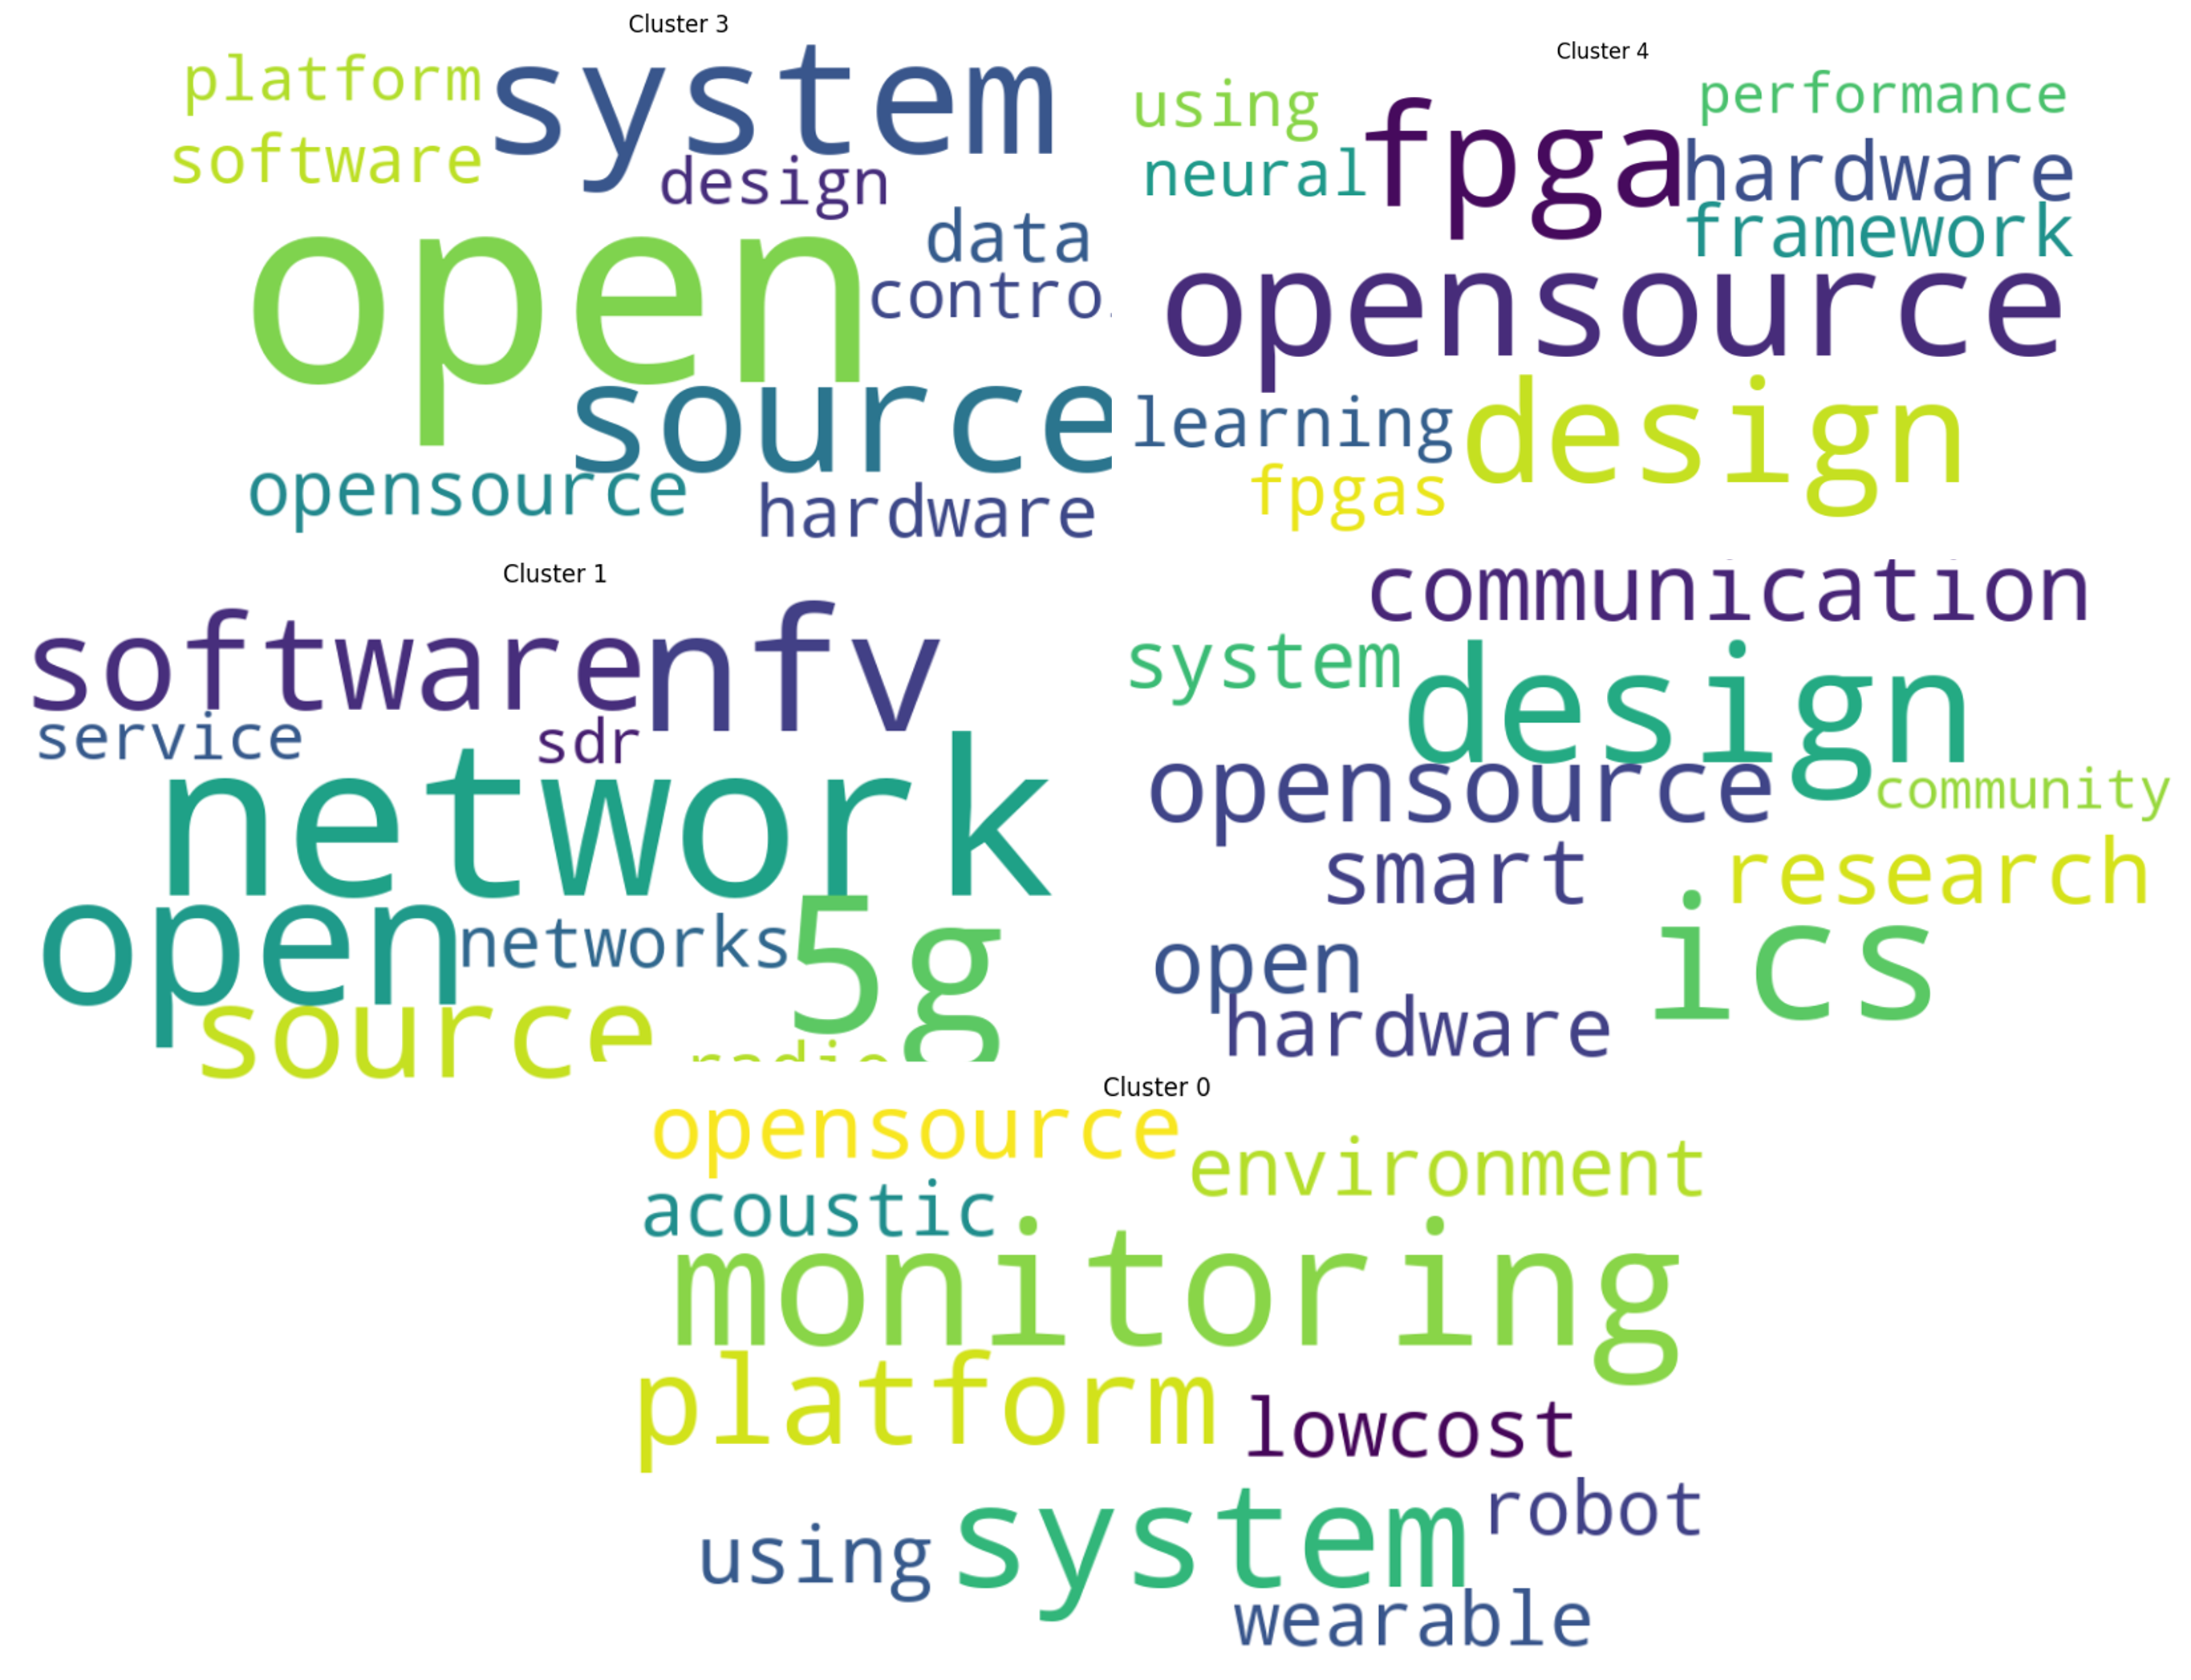
\includegraphics[width=\textwidth]{../Images/wordcloud.png}
        \caption{Word cloud based on the keywords in each cluster.}
        \label{fig:1}
    \end{minipage}
\end{figure}
The development of keywords from 2017 to 2022 can be observed in Fig.(2). Clusters indicate a variety of trends and technological advancements in the field of open-source hardware. In Cluster 0, the focus is on monitoring systems, platforms, and wearable robotics, demonstrating a growing interest in environmental and personal monitoring applications. Cluster 1 highlights the role of network technologies, with 5G, NFV, and SDR being prominent keywords, showcasing the integration of open-source hardware in communication networks and radio systems.

Cluster 2 emphasizes the importance of design and community in the open-source hardware landscape, with a focus on smart communication systems and integrated circuits. This suggests a strong emphasis on collaboration and research in the development of open-source hardware technologies. 

Cluster 3 showcases the interplay between open-source hardware and software, with keywords such as data, control, and platform indicating a broad range of applications and integrations with other technologies.

Finally, Cluster 4 demonstrates the growing relevance of FPGA technology, machine learning, and neural networks in the field of open-source hardware. This indicates that researchers and developers are exploring the potential of open-source hardware to enhance the performance and capabilities of cutting-edge technologies in artificial intelligence and other advanced domains.

Based on the result of the systematic literature review, we can divide the perspective of FOSH in the following categories: electronics and computing, robotics and automation, and education and research.

\begin{figure}[!h]
    \begin{minipage}{0.48\textwidth}
        \centering
        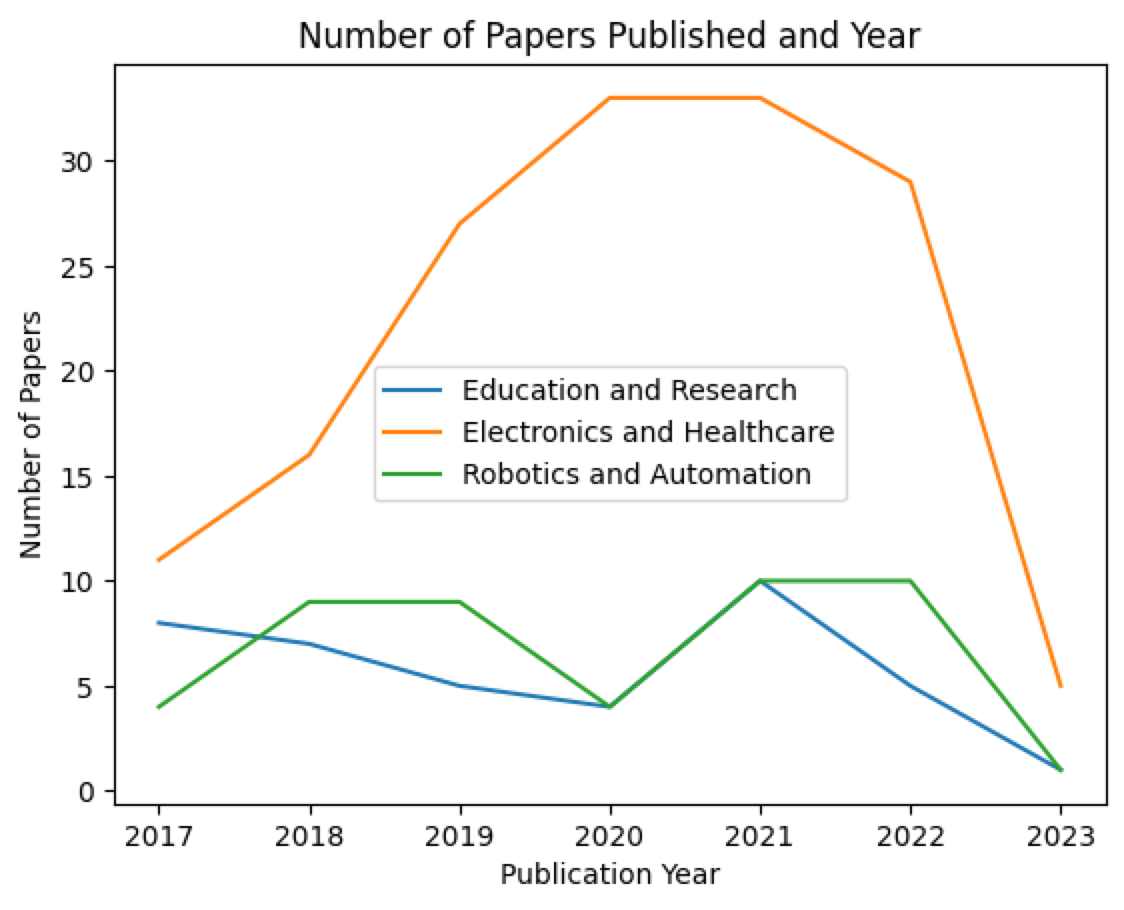
\includegraphics[width=\textwidth]{../Images/num_paper_vs_year.png}
        \caption{Number of papers published in each categories every year}
        \label{fig:1}
    \end{minipage}
\end{figure}
The above figure shows the number of papers published in each year for three different topics, which will be detail explained later. Each topic is represented by a different line color, with a legend indicating which line corresponds to which topic. Note that among the approximately 200 papers, we observed that the majority of papers falls into category "Electronics and Healthcare" compared with the other two. This topic also reaches its high peak between 2020 and 2021, while the other two categories doesn't have a significant difference in number of papers published every year. 


\subsection{Education and Research}

The proliferation of open-source hardware has led to its increasing adoption in educational institutions, ranging from K-12 to graduate programs.\cite{martinez2017open}
This trend can be attributed to the wide applicability of open-source hardware in diverse fields such as electronics\cite{papazoglou2017openhardsim}, computer science, digital media design\cite{chen2021research}, robotics\cite{vrochidou2018open}, and automated vehicles\cite{nakamoto2019development}. 
Taking open-source hardware into courses can provide students with a more comprehensive understanding of the relevant concepts and facilitate hands-on learning experiences.\cite{chen2021research}

Arduino, and Arduino-based platforms, are the most prevalent open-source hardware utilized in schools. 
These tools enable the design of laboratory exercises that target the acquisition of knowledge and skills related to microcontrollers\cite{rankovska2022applying}, microprocessors\cite{papazoglou2017openhardsim}, embedded systems\cite{beneder2017development}, mobile communication networks\cite{lin2017teaching}, optical wireless communications\cite{ahmed2021gr}, and chip design\cite{alam2022open}. 
The versatility and accessibility of open-source hardware make them ideal for fostering a deeper understanding of the basic principles.

What's more, the appearance of new open-source hardware platforms such as the power electronics didactic platform\cite{koleff2019development}, the "ball-on-beam didactic device"\cite{takacs2021bobshield}, the robotic manipulation platform\cite{vcehovin2023low}, and the development of the front-end for the FPGA-based platform\cite{beneder2017development} has further facilitated the teaching and learning of the hardware. 
In addition to the cost-saving benefits, these open-source hardware tools aim to inspire students to contribute to the existing open-source hardware ecosystem. 
As highlighted by V. V. Rankovska et al, the high cost of scientific tools will impede the pace of technological progress. \cite{rankovska2022applying}
Thus, the incorporation of open-source hardware in education can have benefits both in reducing cost and activating the development of the hardware.


\subsection{Electronics and Healthcare}
Some of the most popular and successful hardware are open-sourced, such as Risc-V and Arduino. 
These are free for modification, which is also commonly introduced and extended too various new products. 
For example, Mlakić1 et al. proposed a measurement device implemented based on Arduino \cite{mlakic2019open}. This can be further used to make own IED capable of IoT and smart grid symbiosis. Arduino can also be combined with various products to realize human-computer interaction. 
One example would be Yuning Fan's programming language-based interactive device, which is an interface designed not only for the potential benefit technologically but also to educate children at the same time \cite{fan2021open}. 
As mentioned in the previous paragraph, education is a major field that FOSH is contributing to an strongly impacted in today's community.  
One major reason for any implementation of electronic or computing products is to reduce the cost of the current solution. Noted the vital and complex role of the medical realm, some researches  focus on different fields of this branch. 
For example, the ultrasound test bench demonstrated by Pashaei et al. can be further extended to other devices \cite{pashaei2018live}. 
The key sellout of this product is that it's always in demand for medical equipment, where making the design open-sourced would greatly benefit the whole medical community. 
In addition, given the limitation of availability of affordable medical equipment to treat chronic conditions, Dorin et al. explore the Loop Open-source Artificial Pancreas (APS) \cite{dorin2020open}.
There are similar designs that add convenience for health-related measurement devices such as OpenSenseRT which is also low-cost and extendable, and the robotic platform to enable dexterous procedures within CT scanners which is practically a robot hand that allows physicians to localize tumours quickly \cite{slade2021open}. Robots are another major application area in the FOSH community, which will be further explored in the next paragraph. 

\subsection{Robotics and Automation}
In general, robots are often created to either complete tasks that humans are unable to or to increase productivity. 
VIKTOR III is an open source robot to improve the farming production quality by not only "empower[ing] individuals to grow their own food [but also] serve[ing] as a platform for robotics education".
This also falls into the category of the benefit of open-source products can bring to the field of education. By improving on the current older invention, an open-sourced robot named FarmBot, VIKTOR III can be built only using 1/6 of its cost but with completely the same feature. 
It also uses state-of-art machine learning technology deep learning that provides a higher plant detection accuracy. 
The inventors also suggested that it can help astronauts harvest in space. 
By doing so, it provides a blueprint for future design and study purposes. 
There are many products that share the same goal, such as the Yale OpenHand Project, which focus on improving the design process and producing various options for the researchers to adopt on \cite{ma2017yale}. 
The inventor of WoodenHaptics also agrees with the importance of innovation, which is why they published the blueprint for this design in order to "Lowering the barriers to inspire experimentation" \cite{yip2017spurring}. 
As a realm that is constantly been developed and updated by new technologies, they believe the ultimate future goal for any open-source robot is "identifying willing end users who will put their own design modifications online, thereby allowing progress in the research community to move even faster" \cite{yip2017spurring}. 
In fact, this concept of republishing the modified product is also widely and strongly agreed upon by many researchers, which leads to the invention of ROS\cite{alami2018influencers} (Robot Operating System) that allows people to communicate. 
The aspect of FOSH communities will be further discussed later. 

\subsection{Licences}
There are three pieces of an FOSH that has a licence, the hardware, the software, and the documentation.
The licences can be seen in the tables \ref{tab:hlic}, \ref{tab:slic}, and \ref{tab:dlic}.
The hardware are predominately packaged with a CERN or a derivative of this licence.
The CERN licence also appears in the software and documentation, but it is not the main type. 
Software is packaged with the common MIT licence and the documentation has a common public licence.

\subfile{table_lic.tex}
\sub

\end{document}